\chapter{Termodinámica}
\section{Trabajo}
\begin{enumerate}
\item Durante un \textbf{proceso cuasiestático} un sistema atraviesa 
		en todo momento 
	  estados infinitesimalmente cercanos al equilibrio termodinámico y, 
	  por consiguiente, la dinámica de los estados puede ser descrita
	  en términos de coordenadas termodinámicas $\Rightarrow$ existe 
	  una ecuación de estado que describe estos estados 
\item Equilibrio termodinámico: eq. mecánico $+$ eq. térmico $+$ 
 	  eq. químico
\item Diferencial de trabajo de un sistema de un gas en un pistón:
\begin{equation}
\dbar W= PAdx = -PdV,
\end{equation}
el signo negativo asegura que en una compresión $(dV<0)$ $\dbar W>0$ 
(trabajo sobre el sistema, i.e. el sistema gana energía). 
\item El trabajo realizado sobre un sistema hidrostático depende de 
la trayectoria que se siga en el diagrama de estados (a diferencia
del trabajo realizado por la fuerza gravitacional, por ej). 
\item El trabajo relizado sobre un gas, definido por
\begin{align*}
W=-\int_{V_i}^{V_f} PdV, 
\end{align*}
se puede integrar siempre y cuando se conozca una función 
de estado.
\item ¡¡¡Calor $=$ energía!!!
\end{enumerate}

\section{1era ley de la Termodinámica}
\begin{itemize}
\item Una forma \textbf{restringida} de enunciar la primera ley 
de la termodinámica es:

Si un sistema cerrado es causado a cambiar de estado de un estado 
inicial a un estado final únicamente por procesos adiabáticos, entonces
el trabajo realizado sobre el sistema es el mismo para todas las trayectorias
adiabáticas que conectan a ambos estados. 

Es restringida porque no se está diciendo qué ocurre en 
aquellos procesos no adiabáticos. Es decir, en procesos
en los que ocurre intercambio de calor. 
\item Se sigue de esta forma restringida de la primera ley de la 
Termodinámica que existe una función que depende únicamente
de las coordenadas termodinámicas cuya diferencia entre el valor
final e inicial es igual al trabajo adiabático que se realiza al
sistema pasar del estado inicial al estado final. Esta función 
es la función de \textbf{energía interna} $U$: 
\begin{align}
W_{i\to f}\text{(adiabático)}=U_f-U_i,
\end{align}
esta diferencia da el aumento en energía interna del sistema. 
\item  \textbf{1era. ley de la Termodinámica} (formulación 
matemática): 
Cuando un sistema cerrado y su entorno se encuentran a distintas
temperatura y se realiza trabajo diatérmico [?] sobre el sistema,
entonces la energía transferida por otros procesos no mecánicos, 
igual a la diferencia entre el cambio de energía interna y el 
trabajo diatérmano se llama calor $Q$:
\begin{align}
  \Delta U = Q + W,
  \label{eq:1st-law-thermodynamics}
\end{align}
donde $Q>0$ cuando el calor entra al sistema y $Q<0$ cundo
abandona el sistema. Tres ideas están plasmadas en 
\eqref{eq:1st-law-thermodynamics}: (1) la existencia de una 
función de energía interna, (2) el principio de conservación de 
la energía, y (3) la definición de trabajo como energía en tránsito
en virtud de una diferencia de temperatura.
\item \textbf{Forma diferencial de la 1era. ley de la Termodinámica}:
para un sistema termodinámico que atraviesa cambios infinitesimales 
en sus variables termodinámicas la primera ley se formula como
\begin{align}
  dU = \dbar Q + \dbar W.
  \label{eq:1st-law-thermodynamics_diffForm}
\end{align}
\item \textbf{Capacidad calorífica}: 
\begin{align}
  C=\dv{Q}{T} \qty[\frac{K}{J}]
  \label{eq:heat-capacity}.
\end{align}
\item El caso de un gas:

La ecuación \eqref{eq:1st-law-thermodynamics_diffForm} toma 
la forma 
\begin{align}
   dU =\dbar Q-PdV,
   \label{eq:1st-law-gas}
 \end{align} 
donde $U$ es una función de algún par $P,V,T$ (la ecuación relaciona 
a un par con la tercera). Tomando $U=U(T,V)$ se tiene 
\begin{align*}
dU=\qty(\pdv{U}{T	})_VdT+\qty(\pdv{U}{V})_TdV,
\end{align*}
y sustityendo en \eqref{eq:1st-law-gas}
\begin{align*}
\dbar Q &=\qty(\pdv{U}{T	})_VdT+\qty[\qty(\pdv{U}{V})_T+P]dV\\
\dv{Q}{T} &= \qty(\pdv{U}{T	})_V
+\qty[\qty(\pdv{U}{V})_T+P]\dv{V}{T}.
\end{align*}
\item Flujo cuasiestático de calor: cuando a lo largo de un sistema 
existe un gradiente de temperatura y el calor fluye de manera
cuasiestática (misma definición) podemos calcular el 
calor que se absorbe durante el proceso utilizando la ecuación 
\eqref{eq:heat-capacity} de la capacidad calorífica.
\item El transporte de energía en un sistema entre elementos
de volumen vecinos en virtud de una diferencia de temperatura se 
conoce como conducción de calor. Los experimentos muestran que 
\begin{align*}
\frac{Q}{t}\propto A\frac{\Delta T}{\Delta x},
\end{align*}
con $A$ el área transversal al flujo de calor. Por consiguiente
\begin{align}
\dv{Q}{t	} = -KA\dv{T}{x},
\end{align}
con $K$ la conductividad térmica. El signo menos es para asegurar
que la dirección del flujo de calor sea en la dirección positiva de $x$.
\item \textbf{Radiación térmica}: radiación en virtud de su temperatura.
\item Exitancia radiante $\mathcal{R}$: potencia irradiada total por 
unidad de área. Emisividad total $\epsilon$: fracción de la potencia
irradiada total que es emitida como radiación térmica.
\item \textbf{Ley de Stefan-Boltzmann}: un cuerpo negro es una
sustancia ideal que es capaz de absorber toda la luz incidente 
sobre ella y reemitirla netamente como radiación térmica. La
radiación de un cuerpo como este está dada por la la siguiente ley:
\begin{align}
  \mathcal{R}=\mathcal{R}(T)=\sigma T^4,
  \label{eq:stefan-boltzmann}
\end{align}
donde $\sigma$ es la constante de Stefan-Boltzmann.
\end{itemize}

\section{Gas ideal}
\begin{enumerate}
\item \textbf{Expansión libre adiabática}: gas en expansión en el 
cual no se hace trabajo ni se transfiere calor $\Rightarrow$ $\Delta U=0$
durante la expansión libre.
\item Al escribir explícitamente $dU$ asumiendo que $U=U(T,V)$ ó 
$U=U(T,P)$ y al considerar una expansión libre adiabática $(dU=0)$
se concluye que $U=U(T)$ para un gas ideal. 
\item Un \textbf{gas ideal} satisface
\begin{align}
  PV&=nRT, & \qty(\pdv{U}{P})_T&=0,
  \label{eq:ideal-gas}
\end{align}
la primera condición es la ecuación de estado del gas ideal y 
la segunda es para asegurar que en una expansión libre
$dU=0$.
\item Retomando la ecuación \eqref{eq:1st-law-gas}:
\begin{align*}
\dbar Q=dU+PdV,
\end{align*}
cuando $dV=0$
\begin{align*}
\qty(\dv{Q}{T})_T=C_V=\qty(\pdv{U}{T})_V.
\end{align*}
En el caso del gas ideal $U=U(T)$, por consiguiente
\begin{align*}
C_V=\dv{U}{T},
\end{align*}
y 
\begin{align}
\dbar Q = C_VdT+PdV,
\label{eq:dQ-idealGas}
\end{align}
y sacando un diferencial de la ecuación de estado del gas ideal
\begin{align*}
PdV+VdP=nRdT.
\end{align*}
Sustiyendo arriba
\begin{align*}
\dbar Q &= C_VdT + nRdT - VdP\\
\dv{Q}{T}&=\qty(C_V+nR)-V\dv{P}{T},
\end{align*}
cuando $dP=0$:
\begin{align}
\qty(\dv{Q}{T})_P=C_P=C_V+nR.
\label{eq:C_P-idealGas}
\end{align}
\item \textbf{Procesos adiabáticos del gas ideal:} partimos
de las ecuaciones \eqref{eq:dQ-idealGas} y \eqref{eq:C_P-idealGas}
y consideramos un proceso adiabático $(\dbar Q=0)$,
\begin{align*}
0&=C_VdT+PdV, & 0&=C_PdT-VdP\\
C_VdT&=-PdV, & C_PdT&=VdP,
\end{align*}
dividiendo la ecuación de la derecha entre la de la izquierda
\begin{align}
\frac{C_P}{C_V}&=\gamma=-\frac{V}{P}\dv{P}{V}\nonumber\\
\gamma \frac{dV}{V}&=-\frac{dP}{P} \nonumber\\
\gamma\ln V&=-\ln P+C\nonumber\\
V^{\gamma}&=P^{-1}K \nonumber\\
PV^{\gamma}&=K,
\label{eq:StEq-IdealGas-Adiabatic}
\end{align}
(no hay que ponerle tanto amor a las constantes). Esta  
ecuación es válida para el gas ideal para procesos adiabáticos.
\end{enumerate}

\section{La 2da. ley de la Termodinámica}
Notación:
\begin{itemize}
\item $\abs{Q_H}$: calor intercambiado entre un baño de
alta temperatura y el sistema
\item $\abs{Q_L}$: calor intercambiado entre un baño de 
baja temperatura y el sistema
\item $\abs{W}$: el trabajo intercambiado entre el sistema
y su entorno
\end{itemize}

\begin{itemize}
\item Si $\QH>\QL$ y si $\W$ es realizado por el sistema, 
entonces la máquina que causa que el sistema atraviese
un ciclo se conoce como motor de calor.
\item \textbf{Eficiencia térmica:} 
\begin{align}
\eta=\frac{\W}{\QH}
\label{•}
\end{align}
pero como no hay cambio en la energía interna porque 
el sistema se encuentra en contacto con una fuente de
energía (infinita, de manera idealizada), entonces
\begin{align}
\eta=\frac{\QH-\QL}{\QH}
\label{eq:thermal-eff	}	
\end{align}
\item La transformación de calor en trabajo se consigue 
por dos tipos de motores: los motores de combustión
interna y los motores de combustión externa. La 
transformación ocurre haciendo que un gas atraviese
un ciclo.
\item Motores de combustión interna: motor de gasolina
y diesel.
\item Motores de combustión externa: motor de vapor
y de Stirling.
\item En la \Fref{fig:otto-cycle} se muestra un ciclo de Otto ideal
para un motor de gasolina.
\begin{figure}
  \centering
  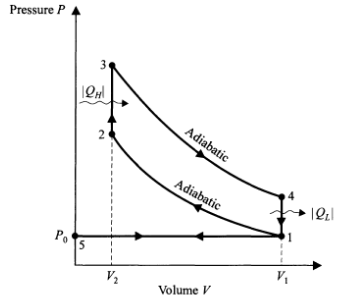
\includegraphics[width=6cm]{images/otto-cycle.png}
  \caption{Ciclo de Otto para un motor de gasolina.}
  \label{fig:otto-cycle}
\end{figure}
\item En la \Fref{fig:diesel-cycle} se muestra un ciclo Diesel ideal.
\begin{figure}
  \centering
  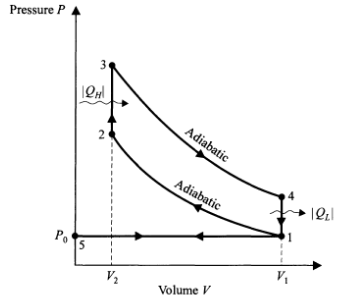
\includegraphics[width=6cm]{images/otto-cycle.png}
  \caption{Ciclo de Diesel ideal.}
  \label{fig:diesel-cycle}
\end{figure}

\begin{figure}
  \centering
  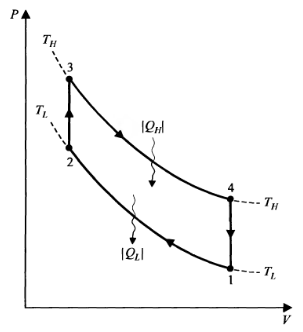
\includegraphics[width=6cm]{images/stirling-cycle.png}
  \caption{Ciclo de Stirling ideal. Nótese que el intercambio 
  de calor entre el sistema y su entorno ocurre sobre curvas
  isotérmicas.}
  \label{fig:diesel-cycle}
\end{figure}
\item Resumen del mecanismo de los motores: 
\begin{itemize}
\item Existe un proceso o conjunto de procesos durante los cuales 
existe absorción de calor de una fuente externa a mayor temperatura.
\item Existe un proceso o conjunto de procesos durante los cuales
el calor es eyectado a una fuente de calor externa a menor 
temperatura.
\end{itemize}
\item \textbf{2da. Ley de la Termodinámica (Kelvin-Planck):} 
Es imposible construir un motor que opere en ciclos y extraiga calor
de una fuente que convierta el calor extraído exclusivamente en trabajo.
\item Un frigorífico es el proceso inverso a un ciclo: (1) se extrae calor
a baja temperatura y (2) se eyecta mucho calor a temperatura alta. En
este ciclo el trabajo es realizado \textbf{sobre} el sistema.
\item \textbf{2da. Ley de la Termodinámica (Clauius):} 
Es imposible construir un frigorífico que, operando en un ciclo, 
transferencia completamente el calor de una fuente 
de menor temperatura a una fuente de temperatura mayor.
\item \janote{Qué pedo con la equivalencia de ambas formas 
de formular 2da ley???? sección 6.8}
\item \textbf{Rerversibilidad e irreversibilidad:} Un proceso 
reversible es un proceso que se realiza de tal forma que el
sistema y su entorno pueden regresar a sus estados iniciales
sin producir ningún cambio en el resto del universo.1
\end{itemize}


\section{Ciclo de Carnot}
\begin{itemize}
\item Ciclo de Carnot: 
\begin{enumerate}
\item Proceso adiabático reversible en la dirección tal que 
la temperatura aumenta hasta la temperatura de la fuente 
de calor caliente a $T_H$.
\item El sistema se mantiene en contacto con la fuente
de calor a $T_H$, y un proceso isotérmico reversible 
toma lugar en dirección y hasta tal punto que 
el calor $\QH$ es absorbido por el sistema desde 
la fuente. 
\item Un proceso adiabático reversible ocurre en dirección 
contraria al proceso 1 hasta que la temperatura baja hasta 
la temperatura de la fuente de calor fría a $T_L$.
\item El sistema se mantiene en contacto con la fuente de 
calor a $T_L$ y un proceso isotérmico reversible toma lugar 
en dirección opuesta al proceso 2 hasta que el sistema y 
su entorno se encuentran en sus estados iniciales. Durante
este proceso el calor $\QL$ sale del sistema hacia la fuente
de temperatura $T_L$.
\begin{figure}
  \centering
  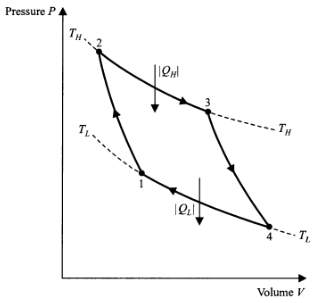
\includegraphics[width=6cm]{images/carnot-cycle.png}
  \caption{Ciclo de Carnot de un gas real.}
  \label{fig:diesel-cycle}
\end{figure}

\newpage

\item \textbf{Teorema de Carnot:} Ningún motor de calor entre
dos fuentes de calor puede ser más eficiente que un motor de
Carnot que opere entre las mismas dos fuentes de calor.
\begin{proof}
Consideremos los siguientes dos ciclos:
\begin{multicols}{2}
\setlength{\columnseprule}{0pt}
\centering
Ciclo de Carnot $R$
\begin{enumerate}
\item Absorbe $\QH$ de la fuente de calor caliente.
\item El sistema realiza el trabajo $\W$
\item El calor $\QH-\W$ se entrega del sistema al entorno.
\item Eficiencia $\eta_R=\W/\QH$
\end{enumerate} 
\columnbreak
\centering
Ciclo de motor irreversible $I$
\begin{enumerate}
\item Absorbe $\abs{Q_H'}$ de la fuente de calor caliente.
\item El sistema realiza el trabajo $\abs{W}$
\item El calor $\abs{Q_H'}-\abs{W}$ se entrega del sistema al entorno.
\item Eficiencia $\eta_I=\abs{W}/\abs{Q_H'}$
\end{enumerate}
\end{multicols}
Asumamos que $\eta_I>\eta_R$, entonces $\QH>\abs{Q_H'}$. Ahora 
consideremos los ciclos inversos. El calor neto que se extrae 
de la fuente de calor fría es $\QH-\abs{Q_H'}$, que es una cantidad
positiva. Sin embargo, también el calor que el sistema entrega
a la fuente caliente es $\QH-\abs{Q_H'}$. Por lo tanto, el sistema
(un frigorífico) estaría transfiriendo todo el calor extraído de una 
fuente de calor fría hacia una fuente de calor caliente, lo cual 
viola la segunda ley de la Termodinámica. 
\end{proof}
\end{enumerate}
\end{itemize}

\section{Entropía}
\begin{itemize}
\item Para cualquier ciclo reversible se cumple que
\begin{align}
\oint_R \dv{Q}{T}=0.
\label{eq:clausius-theo}
\end{align}
Este resultado es conocido como el teorema de Clausius.

\item \textbf{Entropía}
\begin{figure}
  \centering
  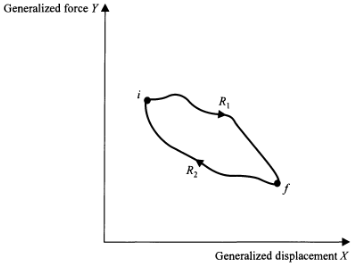
\includegraphics[width=6cm]{images/reversible-paths.png}
  \caption{Dos caminos reversibles uniendo dos estados de equilibrio
  de un sistema.}
  \label{fig:reversible-paths}
\end{figure}
Consideremos un sistema como el que describe la \Fref{fig:reversible-paths}. 
Del teorema de Clausius, \eqref{eq:clausius-theo},
\begin{align*}
\sideset{_{R_1R_2}}{}\oint \dv{Q}{T}&=
\sideset{_{R_1}}{_i^f}\int \dv{Q}{T} 
+\sideset{_{R_2}}{_f^i}\int \dv{Q}{T}=0\\
\sideset{_{R_1}}{_i^f}\int \dv{Q}{T} &=-\sideset{_{R_2}}{_f^i}\int \dv{Q}{T},
\end{align*}
pero como $R_2$ es un camino reversible
\begin{align*}
-\sideset{_{R_2}}{_f^i}\int \dv{Q}{T} = \sideset{_{R_2}}{_i^f}\int \dv{Q}{T},
\end{align*}
por lo tanto 
\begin{align}
\sideset{_{R_1}}{_i^f}\int \dv{Q}{T} &=\sideset{_{R_2}}{_i^f}\int \dv{Q}{T}.
\end{align}
De esta ecuación se deriva que existe una función de variables 
termodinámicas de un sistema cuya diferencia entre sus 
valores final menos inicial es igual a la integral $\sideset{_R}{_i^f}\int
\dbar Q/T$: la función de entropía $S$,
\begin{align}
S_f-S_i&=
\sideset{_R}{_i^f}\int \dv{Q}{T},
\end{align}
por lo cual el cambio en la entropía $\Delta S$ es independiente
del camino reversible que tome el sistema. Esto de forma diferencial,
para dos estados inicial y final infinitesimalmente juntos, esta ecuación 
se vuelve
\begin{align}
dS=\frac{\dbar Q_R}{T},
\end{align}
el subíndice $R$ enfatiza que el $\dbar Q$ se transfiera de manera 
reversible.
\item \textbf{Principio de Carathéodory:} 
En la vecindad de cualquier estado inicial $P_0$ de un sistema
físico, existen estados vecinos que son inaccesibles desde $P_0$ 
llegando a ellos a lo largo de trayectorias cuasi estáticas adiabáticas.
\item \textbf{Proceso iseontrópico:} $dS=0\rightarrow S=\text{cte.}$
\item \textbf{Enunciado matemático de Clausius de la 
2da. ley de la Termodinámica:}
\begin{align}
\oint \dv{Q}{T}\leq 0
\end{align}
\item \textbf{En general,}
\begin{align}
dS \geq \dv{Q}{T},
\label{eq:general-dS}
\end{align}
donde la igualdad se cumple para procesos reversibles y la
desigualdad para procesos irreversibles. \janote{Esta vaina me parece
sumamente importante, como que va cerrando el marco teórico de
la 2da ley. Bárbaro ese Clausius}
\item \textbf{Principio de entropía:} $\Delta S(\text{universo})\geq0$ 
(también una consecuencia de la 2da ley de la Termodinámica)
\begin{figure}
  \centering
  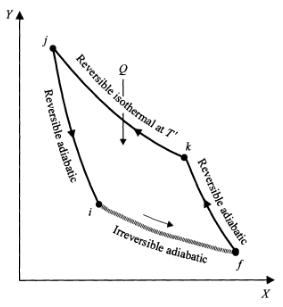
\includegraphics[width=6cm]{images/entropy-principle.png}
  \caption{Un ciclo que contradice la 2da. ley de la Termodinámica
  a menos que $S_f>S_i$.}
  \label{fig:reversible-paths}
\end{figure}
\end{itemize}
\section{Métodos matemáticos}
\begin{itemize}
\item \textbf{Transformaciones diferenciales de Legendre:} 
Si el estado de un sistema está descrito por una función 
de dos variables $\mathbf{f(x,y)}$, que satisface la ecuación
\begin{align}
df=udx+vdy
\label{eq:df-Legendre}	
\end{align}
y deseamos cambiar la descripción a una que involucre
una nueva función $\mathbf{g(u,y)}$, que satisfaga una 
ecuación similar en términos de $du$ y $dy$, entonces
es necesario definir una \textbf{transformación
de Legendre} $g(u,y)$ como 
\begin{align}
g\equiv f-ux.
\label{eq:Legendre-transformation}
\end{align}
La función $g$ debe satisfacer
\begin{align}
\mathbf{dg=-xdu+vdy}.
\end{align}
\item Usemos la transformación de Legendre para definir
nuevas funciones de estado. Primero, la entalpía $H\equiv U+PV$.
Como $U$, $P$ y $V$ son funciones de estados, también lo es $H$.
En forma diferencial, siguiendo la transformación de Legendre:
\begin{align}
dH=VdP+TdS
\end{align}
\item Relaciones diferenciales de las 4 funciones de estado:
\begin{align}
dU = -PdV+TdS\nonumber\\
dH=VdP+TdS \label{eq:diff-form-eq-state}\\
dA=-PdV-SdT\nonumber\\
dG=VdP-SdT\nonumber
\end{align}
\item \textbf{Entalpía:}  
\begin{align*}
dH-dU&=VdP+PdV\\
dH&=dU+VDP+PdV\\
dH&=dQ+VdP,
\end{align*}
cuando $dQ=0$:
\begin{align*}
\Delta H=\int VdP,
\end{align*}
y cuando $dP=0$:
\begin{align*}
\Delta H=\int dQ=\int C_PdT \text{Calor latente [?]}
\end{align*}
\item \textbf{Dos teoremas matmáticos:} (encaminados a 
las relaciones de Maxwell)
\begin{teorema}[\label{teo:1}]
Si 
\begin{align*}
dz=\qty(\pdv{z}{x})_ydx+\qty(\pdv{z}{y})_xdy,
\end{align*}
y tomamos 
\begin{align*}
M&=\qty(\pdv{z}{x})_y & N&=\qty(\pdv{z}{y})_x,
\end{align*}
entonces $z$, $M$ y $N$ son funciones de $x$ y $y$. Se cumple que
\begin{align*}
\pdv{M}{y}&=\qty(\pdv{z}{x}{y})_x & 
\pdv{N}{x}&=\qty(\pdv{z}{y}{x})_y,
\end{align*}
ya que el lado derecho de ambas ecuaciones es igual entonces se 
sigue que 
\begin{align}
\qty(\pdv{M}{y})_x=\qty(\pdv{N}{x})_y.
\end{align}
Esto se conoce como la condición para un diferencial exacto y 
se aplica para las cuatro funciones $U$, $H$, $A$ y $G$.
\end{teorema}
\begin{teorema}
Supongamos una función $f=f(x,y,z)$. Entonces considerando
$x=x(f,y)$ y $y=y(f,z)$
\begin{align*}
dx&=\qty(\pdv{x}{f})_ydf+\qty(\pdv{x}{y})_fdy\\
dy&=\qty(\pdv{y}{f})_zdf+\qty(\pdv{y}{z})_fdz,
\end{align*}
sustityendo la segunda ecuación en la primera
\begin{align*}
dx&=\qty(\pdv{x}{f})_ydf+\qty(\pdv{x}{y})_f
\qty(\qty(\pdv{y}{f})_zdf+\qty(\pdv{y}{z})_fdz),
\end{align*}
pero 
\begin{align*}
dx=\qty(\pdv{x}{f})_zdf+\qty(\pdv{x}{z})_fdz.
\end{align*}
Igualando $dz$ de las últimas dos ecuaciones tenemos 
\begin{align}
\qty(\pdv{x}{y})_f\qty(\pdv{y}{z})_f=\qty(\pdv{x}{z})_f,
\end{align}
lo que significa que 
\begin{align}
\qty(\pdv{x}{y})_f\qty(\pdv{y}{z})_f\qty(\pdv{z}{x})_f=1.
\end{align}
Además, igualando las mismas ecuaciones para $df$
\begin{align}
\qty(\pdv{x}{f})_z=
\qty(\pdv{x}{f})_y+\qty(\pdv{x}{y})_f\qty(\pdv{y}{f})_z.
\end{align}
\end{teorema}
\end{itemize}
\subsection{Relaciones de Maxwell}
\janote{Creo que esta sección, junto con las 
3 leyes debería ser lo más importante de Termo\newline}
Teniendo en mente de nuevo la forma diferencial de las
ecuaciones de estado
\begin{align*}
dU = -PdV+TdS\\
dH=VdP+TdS \\
dA=-PdV-SdT\\
dG=VdP-SdT,
\end{align*}
y usando el teorema \eqref{teo:1} se tiene
\begin{align}
-\qty(\pdv{P}{S})&=\qty(\pdv{T}{V}) \\
\qty(\pdv{T}{P})&=\qty(\pdv{V}{S}) \\
\qty(\pdv{S}{V})&=\qty(\pdv{P}{T}) \\
-\qty(\pdv{S}{P})&=\qty(\pdv{V}{T}),
\end{align}
que se conocen como las \h{\textbf{relaciones de Maxwell}}.
Estas ecuaciones expresan relaciones que se cumplen 
para cualquier estado de equilibrio de un sistema hidrostático.
\begin{figure}[H]
  \centering
  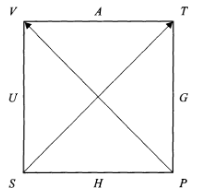
\includegraphics[width=5cm]{images/vat-vus.png}
  \caption{Para recordar más fácil las relaciones de Maxwell.}
  \label{fig:vat-vus}
\end{figure}

\subsection{Ecuaciones $TdS$}
Considerando la función de entropía $S$ dependiente de 
distintos pares de variables termodinámicas $T,V,P$ se pueden 
obtener las ecuaciones $TdS$. 
\begin{itemize}
\item \textbf{Primera ecuación $TdS$:} $(S=S(T,V))$
\begin{align}
TdS=C_VdT+T\qty(\pdv{P}{V})_VdV
\end{align}
\item \textbf{Segunda ecuación $TdS$:} $(S=S(T,P)$
\begin{align}
TdS=C_PdT-T\qty(\pdv{V}{T})_PdP
\end{align}
\end{itemize}

\subsection{Ecuaciones de la energía interna}
\begin{itemize}
\item \textbf{Primera ecuación de la energía interna:}
\begin{align}
\qty(\pdv{U}{V})_T=T\qty(\pdv{P}{T})_V-P
\end{align}
\item \textbf{Segunda ecuación de la energía interna:}
\begin{align}
\qty(\pdv{U}{P})_T=T\qty(\pdv{V}{T})_P-P\qty(\pdv{V}{P})_T
\end{align}
\end{itemize}








